%!TEX TS-program = tectonic
\documentclass[10pt]{article}

\usepackage[paperwidth=7in,paperheight=10in,top=.70in,bottom=.70in,left=.68in,right=.68in,headheight=18pt,headsep=15pt,footskip=25pt]{geometry}
\usepackage{fontspec}
\usepackage[nopatch=footnote]{microtype}
\usepackage{amsmath,amssymb}
\usepackage{xcolor}
\usepackage{tikz}
\usetikzlibrary{calc,positioning,arrows.meta,backgrounds,fit,shapes.geometric}
\usepackage[skins,breakable]{tcolorbox}
\usepackage{enumitem}
\usepackage{fancyhdr}
\usepackage{multicol}
\usepackage{ragged2e}
\usepackage{hyperref}
\usepackage{parskip}
\usepackage{needspace}

\defaultfontfeatures{Ligatures=TeX,Scale=MatchLowercase}
\setmainfont{Iowan Old Style}
\setsansfont{Avenir Next}[Scale=.93]
\setmonofont{Menlo}[Scale=.80]

\definecolor{Void}{HTML}{070A0F}
\definecolor{Deep}{HTML}{0A0E15}
\definecolor{Panel}{HTML}{101620}
\definecolor{PanelTwo}{HTML}{141B25}
\definecolor{Bone}{HTML}{F1ECE3}
\definecolor{Muted}{HTML}{A4A3A0}
\definecolor{Dim}{HTML}{656A73}
\definecolor{Grid}{HTML}{222A36}
\definecolor{Gold}{HTML}{D6A647}
\definecolor{Oxide}{HTML}{C86136}
\definecolor{Green}{HTML}{38A873}
\definecolor{Violet}{HTML}{8E68C9}
\definecolor{Blue}{HTML}{3488B0}
\definecolor{Teal}{HTML}{20A090}
\definecolor{Steel}{HTML}{607FA2}
\definecolor{Red}{HTML}{C64040}
\definecolor{Parchment}{HTML}{F4F0E7}
\definecolor{ClayPaper}{HTML}{F2E6DE}
\definecolor{TealPaper}{HTML}{E2EFED}
\definecolor{GoldPaper}{HTML}{F2EAD8}
\definecolor{GreenPaper}{HTML}{E5EEE6}
\definecolor{BluePaper}{HTML}{E1EBEE}
\definecolor{VioletPaper}{HTML}{ECE6F2}
\definecolor{Ink}{HTML}{171B22}
\definecolor{LightMuted}{HTML}{555C62}

\pagecolor{Void}
\color{Bone}
\hypersetup{colorlinks=true,linkcolor=Gold,urlcolor=Gold,pdfauthor={E.T. Ellis},pdftitle={The RCCX-Hunter-Dabrowski Cascade Model: Visual Atlas v3.2}}

\setlength{\parindent}{0pt}
\setlength{\parskip}{.52em}
\linespread{1.05}
\emergencystretch=2em
\setlist[itemize]{leftmargin=1.18em,itemsep=.18em,topsep=.25em,parsep=0pt,label=\textcolor{Gold}{\tiny$\blacktriangleright$}}

\newcommand{\track}[1]{\addfontfeatures{LetterSpace=#1}}
\newcommand{\CurrentField}{FIELD ATLAS}
\newcommand{\FieldColor}{Gold}
\newcommand{\setfield}[2]{\renewcommand{\CurrentField}{#1}\renewcommand{\FieldColor}{#2}}
\newcommand{\status}[2]{\textsf{\fontsize{6.3}{7}\selectfont\bfseries\track{70}\textcolor{#2}{#1}}}
\newcommand{\kicker}[1]{{\sffamily\fontsize{7.1}{9}\selectfont\bfseries\track{135}\textcolor{\FieldColor}{#1}}\par}
\newcommand{\fieldtitle}[1]{\Needspace{5\baselineskip}\vspace{.25em}{\sffamily\bfseries\fontsize{20}{23}\selectfont #1}\par\vspace{.12em}{\color{\FieldColor}\rule{.82in}{2.1pt}}\par\vspace{.35em}}
\newcommand{\subhead}[1]{\Needspace{3\baselineskip}\vspace{.32em}{\sffamily\bfseries\fontsize{10.3}{12}\selectfont\textcolor{\FieldColor}{#1}}\par\vspace{-.08em}}
\newcommand{\axiom}[1]{\begin{center}\begin{minipage}{.88\linewidth}{\color{\FieldColor}\rule{.34in}{2pt}}\par\vspace{.32em}{\fontsize{13.3}{17}\selectfont\itshape #1}\par\vspace{.34em}{\color{\FieldColor}\rule{.34in}{2pt}}\end{minipage}\end{center}}

\newtcolorbox{fieldcard}[3][]{
  enhanced,breakable,frame hidden,colback=white,opacityback=0,coltext=Ink,boxrule=0pt,arc=0mm,
  left=11pt,right=3pt,top=3pt,bottom=4pt,before skip=9pt,after skip=10pt,
  borderline west={2.4pt}{0pt}{#2},
  title={#3},fonttitle=\sffamily\bfseries\fontsize{11}{13}\selectfont,
  coltitle=#2,attach title to upper={\par\vspace{2pt}},#1
}
\newtcolorbox{evidencebox}[2][]{
  enhanced,colback=Deep,colframe=#2!75!Void,coltext=Bone,boxrule=.5pt,arc=1.5mm,
  left=7pt,right=7pt,top=6pt,bottom=6pt,before skip=5pt,after skip=5pt,#1
}

\pagestyle{fancy}
\fancyhf{}
\fancyhead[L]{\sffamily\bfseries\fontsize{7}{8}\selectfont\track{125}\textcolor{\FieldColor}{\CurrentField}}
\fancyhead[R]{\sffamily\fontsize{7}{8}\selectfont\textcolor{Dim}{RCCX--HUNTER--D\k{A}BROWSKI CASCADE · v3.2}}
\fancyfoot[L]{\sffamily\fontsize{6.8}{8}\selectfont\textcolor{Dim}{WORKING THEORETICAL FRAMEWORK · E.T. ELLIS}}
\fancyfoot[R]{\sffamily\bfseries\fontsize{8}{9}\selectfont\textcolor{\FieldColor}{\thepage}}
\renewcommand{\headrulewidth}{0pt}
\renewcommand{\footrulewidth}{0pt}

\newcommand{\fieldbackground}[1]{%
\begin{tikzpicture}[remember picture,overlay]
  \fill[Void] (current page.north west) rectangle (current page.south east);
  \foreach \y in {0.8,1.6,...,9.6}{\draw[Grid!55,line width=.25pt] ([yshift=-\y in]current page.north west)--([yshift=-\y in]current page.north east);}
  \fill[#1,opacity=.055] ([xshift=-1.0in,yshift=-1.1in]current page.north east) circle (2.4in);
\end{tikzpicture}}
\newcommand{\lightfieldbackground}[2]{%
\color{Ink}%
\begin{tikzpicture}[remember picture,overlay]
  \fill[#2] (current page.north west) rectangle (current page.south east);
  \foreach \y in {0.8,1.6,...,9.6}{\draw[Ink,opacity=.10,line width=.28pt] ([yshift=-\y in]current page.north west)--([yshift=-\y in]current page.north east);}
  \fill[#1,opacity=.07] ([xshift=-1.0in,yshift=-1.1in]current page.north east) circle (2.4in);
\end{tikzpicture}}

\begin{document}
\raggedbottom
\hypersetup{pageanchor=false}

% COVER — stratified substrate, living loop, and bifurcating future.
\begin{titlepage}
\thispagestyle{empty}
\begin{tikzpicture}[remember picture,overlay]
  \fill[Void] (current page.north west) rectangle (current page.south east);
  \foreach \y/\c in {0.0/Gold,0.16/Oxide,0.32/Green,0.48/Violet,0.64/Blue,0.80/Teal}{
    \draw[\c,opacity=.55,line width=.55pt] ([xshift=.48in,yshift=\y in]current page.south west) .. controls ([xshift=2.0in,yshift=\y in+.22in]current page.south west) and ([xshift=3.0in,yshift=\y in-.16in]current page.south west) .. ([xshift=4.6in,yshift=\y in]current page.south west);
  }
  \coordinate (spine) at ([xshift=-1.52in,yshift=.18in]current page.center);
  \draw[Bone!18,line width=.6pt] ([yshift=3.05in]spine)--([yshift=-2.25in]spine);
  \foreach \yy/\c/\r in {2.75/Gold/3.5,2.05/Green/3.0,1.32/Violet/3.0,.52/Blue/3.0,-.25/Oxide/3.3,-1.02/Teal/3.2,-1.72/Gold/3.8}{
    \fill[\c] ([yshift=\yy in]spine) circle (\r pt);
    \draw[\c,opacity=.22] ([yshift=\yy in]spine) circle (.34in);
  }
  \coordinate (fork) at ([yshift=-2.25in]spine);
  \draw[Red,line width=1.1pt] (fork)--++(-1.15in,-.72in);
  \draw[Green,line width=1.1pt] (fork)--++(1.15in,-.72in);
  \fill[Red] ($(fork)+(-1.15in,-.72in)$) circle (3pt);
  \fill[Green] ($(fork)+(1.15in,-.72in)$) circle (3pt);
  \draw[Gold,opacity=.65,line width=1.1pt,-{Stealth[length=6pt]}] ($(fork)+(1.15in,-.72in)$)--++(.72in,-.60in);
  \draw[Gold,opacity=.36,line width=.8pt] ([xshift=1.18in,yshift=-.55in]current page.center) circle (1.58in);
  \draw[Gold,opacity=.18,line width=.45pt] ([xshift=1.18in,yshift=-.55in]current page.center) circle (1.10in);
  \foreach \a in {15,58,103,151,204,252,301,344}{
    \draw[Teal,opacity=.30,line width=.45pt] ([xshift=1.18in,yshift=-.55in]current page.center)--++(\a:2.05in);
    \fill[Bone!80] ($([xshift=1.18in,yshift=-.55in]current page.center)+(\a:2.05in)$) circle (1.7pt);
  }
\end{tikzpicture}

\vspace*{.42in}
{\sffamily\bfseries\fontsize{7.5}{9}\selectfont\track{190}\textcolor{Gold}{INTEGRATED CAUSAL FIELD · VISUAL ATLAS v3.2}}\par
\vspace{.44in}
{\sffamily\bfseries\fontsize{28}{30}\selectfont THE RCCX--HUNTER--\\D\k{A}BROWSKI CASCADE}\par
\vspace{.22in}{\color{Oxide}\rule{1.2in}{3pt}}\par
\vspace{.22in}
{\fontsize{12.4}{17}\selectfont\itshape\color{Bone!90}
A layered model of constitutional sensitivity, regulatory coupling, developmental bifurcation, and the conversion of latent capacity into historically legible output.}\par

\vfill
\begin{minipage}{.74\linewidth}
{\fontsize{11.7}{16}\selectfont
The phenotype is not the diagnosis. The diagnosis is one readout of a coupled system whose body, environment, developmental history, attention, identity, and available conversion surfaces keep acting back upon one another.}
\end{minipage}

\vspace{.42in}
{\sffamily\bfseries\fontsize{8.8}{10}\selectfont\track{105}\textcolor{Gold}{E.T. ELLIS}}\hfill
{\sffamily\fontsize{7.4}{9}\selectfont\textcolor{Dim}{v3.2 · SEPTEMBER 2026}}
\end{titlepage}

\hypersetup{pageanchor=true}
\pagenumbering{arabic}

% MASTER PLATE
\setfield{MASTER FIELD}{Gold}
\lightfieldbackground{Gold}{Parchment}
\kicker{THE WHOLE MODEL}
\fieldtitle{One Cascade, Multiple Certainty Levels}

{\small\color{LightMuted}Nodes name layers. Badges grade claim status. Line styles distinguish directional mechanism from proposed modulation and recursive feedback. The diagram is a map of a research program, not a claim that every arrow has already been proven.}\par

\begin{center}
\resizebox{\textwidth}{!}{%
\begin{tikzpicture}[
  x=1in,y=.55in,
  node distance=.25in,
  flow/.style={draw=#1,fill=Panel,rounded corners=3pt,minimum height=.42in,text width=2.07in,align=center,font=\sffamily\bfseries\fontsize{7.6}{9}\selectfont,text=Bone},
  smallflow/.style={draw=#1,fill=Panel,rounded corners=3pt,minimum height=.36in,text width=1.75in,align=center,font=\sffamily\bfseries\fontsize{7}{8}\selectfont,text=Bone},
  mech/.style={-{Stealth[length=5pt]},line width=.75pt,draw=Muted},
  proposal/.style={-{Stealth[length=5pt]},line width=.75pt,dashed,draw=Gold!80},
  feedback/.style={-{Stealth[length=5pt]},line width=.7pt,densely dashed,draw=Green!75}
]
\node[smallflow=Gold] (rccx) at (-1.25,0) {RCCX constitutional cluster\\[-1pt]\normalfont\fontsize{5.7}{6.5}\selectfont PROPOSED SUBSTRATE};
\node[smallflow=Oxide] (hunter) at (1.25,0) {Hunter--Farmer mismatch\\[-1pt]\normalfont\fontsize{5.7}{6.5}\selectfont ECOLOGICAL LENS};
\node[flow=Green] (epi) at (0,-1.15) {Epigenetic regulation};
\node[flow=Violet] (oe) at (0,-2.15) {D\k{a}browski overexcitabilities};
\node[flow=Blue] (env) at (0,-3.15) {Early developmental environment};
\node[smallflow=Red] (stress) at (0,-4.15) {Chronic stress / C-PTSD};
\node[flow=Oxide] (ans) at (0,-5.15) {Autonomic set-point reorganization};
\node[flow=Teal] (attn) at (0,-6.15) {State-dependent attention};
\node[flow=Steel] (mask) at (0,-7.15) {Homeostatic masking};
\node[flow=Violet] (social) at (0,-8.15) {Social misreading + rejection sensitivity};
\node[draw=Muted,fill=Deep,diamond,aspect=4.6,inner sep=2pt,align=center,font=\sffamily\bfseries\fontsize{6.8}{8}\selectfont,text=Bone] (bif) at (0,-9.35) {DEVELOPMENTAL REORGANIZATION};
\node[smallflow=Red] (frag) at (-1.25,-10.55) {Fragmenting reorganization};
\node[smallflow=Green] (coh) at (1.25,-10.55) {Coherent reorganization};
\node[flow=Gold] (toggles) at (1.25,-11.72) {Three-toggle convergence};
\node[smallflow=Gold] (history) at (1.25,-12.82) {Historically legible output};

\draw[proposal] (rccx)--(epi); \draw[proposal] (hunter)--(epi);
\draw[proposal] (epi)--(oe); \draw[mech] (oe)--(env); \draw[mech] (env)--(stress);
\draw[mech] (stress)--(ans); \draw[proposal] (ans)--(attn); \draw[mech] (attn)--(mask);
\draw[mech] (mask)--(social); \draw[mech] (social)--(bif);
\draw[-{Stealth[length=5pt]},draw=Red,line width=.8pt] (bif)--(frag);
\draw[-{Stealth[length=5pt]},draw=Green,line width=.8pt] (bif)--(coh);
\draw[-{Stealth[length=5pt]},draw=Gold,line width=.85pt] (coh)--(toggles);
\draw[-{Stealth[length=5pt]},draw=Gold,line width=.85pt] (toggles)--(history);
\draw[feedback] (ans.west) to[out=190,in=170,looseness=1.1] node[left,font=\ttfamily\fontsize{5.3}{6}\selectfont,text=Green,align=center]{PHYSIOLOGICAL\\FEEDBACK} (oe.west);
\draw[feedback] (social.west) to[out=190,in=170,looseness=1.05] node[left,font=\ttfamily\fontsize{5.3}{6}\selectfont,text=Green,align=center]{INTERGENERATIONAL\\LOOP} (env.west);

\node[draw=Gold,fill=Deep,rounded corners=5pt,text width=1.48in,minimum height=2.0in,align=left,font=\fontsize{6.4}{8}\selectfont,text=Muted] (rco) at (3.25,-5.7) {\textcolor{Gold}{\sffamily\bfseries REGULATORY COUPLING ORIENTATION}\\[4pt]\textcolor{Bone}{External-cue dominant}\\novelty · motion · urgency\\[5pt]\textcolor{Bone}{Internally sustained}\\routine · delayed reward\\[6pt]\textcolor{Teal}{ADHD-like dynamics}\\readout + gain term};
\draw[proposal] (attn.east)--(rco.west);
\draw[proposal] (rco.west) to[out=170,in=10] (ans.east);
\end{tikzpicture}
}
\end{center}

\vfill
\begin{center}{\sffamily\fontsize{6.6}{8}\selectfont
\textcolor{LightMuted}{SOLID} directional mechanism \quad
\textcolor{Gold}{DASHED} proposed modulation \quad
\textcolor{Green}{LOOPED} recursive feedback}\end{center}

\clearpage

% MOVEMENT I
\setfield{MOVEMENT I · CONSTITUTION}{Gold}
\lightfieldbackground{Gold}{Parchment}
\kicker{SUBSTRATE / ECOLOGY / DEVELOPMENTAL POTENTIAL}
\fieldtitle{Constitution Is a Constraint, Not a Destiny}

\begin{fieldcard}{Gold}{RCCX constitutional cluster \hfill \status{PROPOSED CLUSTER}{Gold}}
\textcolor{LightMuted}{\small A candidate organizing substrate, not a settled genotype-to-phenotype map.}
\begin{itemize}
  \item C4 · CYP21A2 · TNXB linkage-region proposal.
  \item Connective-tissue, immune, endocrine, and stress-axis convergence.
  \item The hypothesis concerns a constitutional probability field. It does not assign one inevitable phenotype to one genotype.
\end{itemize}
\end{fieldcard}

\begin{fieldcard}{Oxide}{Hunter--Farmer mismatch lens \hfill \status{EVOLUTIONARY LENS}{Oxide}}
\textcolor{LightMuted}{\small Ecology changes the functional value of the same regulatory tendencies.}
\begin{itemize}
  \item Broad scanning, change detection, rapid response, and active sampling may fit variable, immediate-feedback environments.
  \item The same tendencies may become costly inside low-variance, delayed-reward institutions.
  \item Hunter and Farmer are ecological renderings of a deeper regulatory architecture, not permanent human types.
\end{itemize}
\end{fieldcard}

\begin{fieldcard}{Green}{Epigenetic regulation \hfill \status{SUPPORTED MECHANISM}{Green}}
Developmental environments can tune HPA-axis and glucocorticoid signaling without changing DNA sequence. Similar constitutional profiles may diverge through developmental marking. Intergenerational associations exist, but their transmission pathways remain bounded and must not be overstated.
\end{fieldcard}

\begin{fieldcard}{Violet}{D\k{a}browski overexcitabilities \hfill \status{DEVELOPMENTAL THEORY}{Violet}}
Five high-gain channels expand both possibility and effective dose:
\begin{center}\small
\textcolor{Oxide}{psychomotor} · \textcolor{Blue}{sensory} · \textcolor{Red}{emotional} · \textcolor{Teal}{intellectual} · \textcolor{Violet}{imaginational}
\end{center}
Movement pressure, intensified sensory intake, amplified affective signal, recursive analysis, and high-throughput counterfactual generation can raise developmental potential. They can also increase the amount of environment the organism must metabolize.
\end{fieldcard}

\axiom{The same high-gain substrate can raise the ceiling and raise the cost of remaining organized enough to reach it.}

\clearpage

% MOVEMENT II — DEVELOPMENTAL BODY
\setfield{MOVEMENT II · REGULATION}{Oxide}
\lightfieldbackground{Oxide}{ClayPaper}
\kicker{ENVIRONMENT WRITES INTO STATE}
\fieldtitle{The Body Becomes Part\\of the Historical Record}

\begin{fieldcard}{Blue}{Early developmental environment \hfill \status{ESTABLISHED DOMAIN}{Blue}}
Constitution meets reinforcement, attachment, threat, social fit, and institutional structure. Inconsistent reinforcement, emotional neglect, covert threat cues, and low-fit environments do not merely surround regulation. Environmental variance becomes part of the regulatory circuit itself.
\end{fieldcard}

\begin{center}
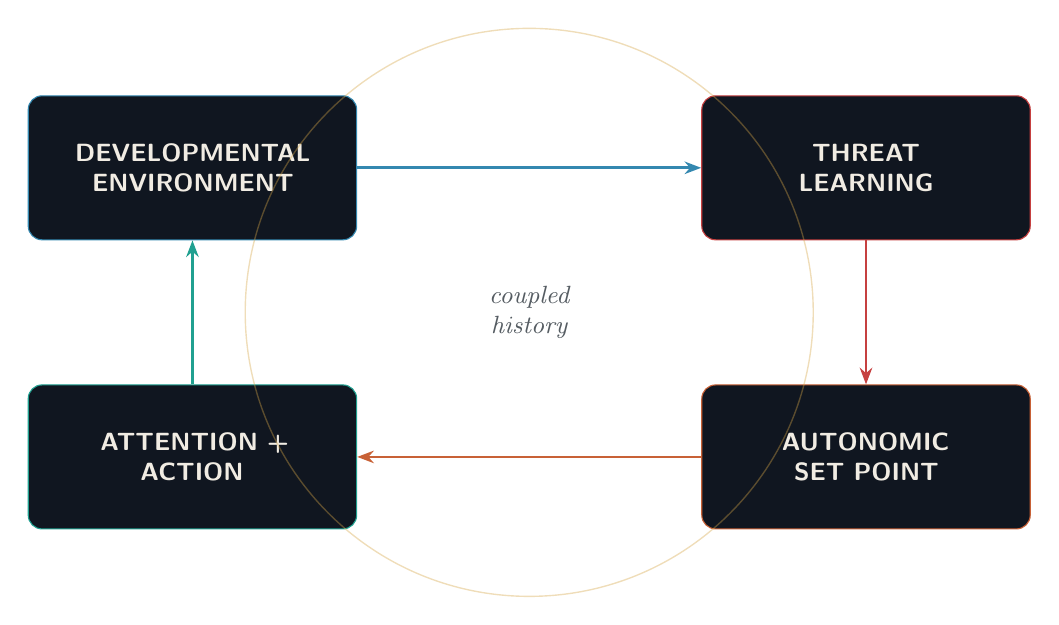
\begin{tikzpicture}[node distance=.48in]
\node[draw=Blue,fill=Panel,text=Bone,rounded corners=5pt,text width=1.55in,minimum height=.72in,align=center,font=\sffamily\bfseries\small] (env) {DEVELOPMENTAL\\ENVIRONMENT};
\node[draw=Red,fill=Panel,text=Bone,rounded corners=5pt,text width=1.55in,minimum height=.72in,align=center,font=\sffamily\bfseries\small,right=1.72in of env] (threat) {THREAT\\LEARNING};
\node[draw=Oxide,fill=Panel,text=Bone,rounded corners=5pt,text width=1.55in,minimum height=.72in,align=center,font=\sffamily\bfseries\small,below=.72in of threat] (body) {AUTONOMIC\\SET POINT};
\node[draw=Teal,fill=Panel,text=Bone,rounded corners=5pt,text width=1.55in,minimum height=.72in,align=center,font=\sffamily\bfseries\small,left=1.72in of body] (attention) {ATTENTION +\\ACTION};
\draw[-{Stealth[length=6pt]},Blue,line width=1pt] (env)--(threat);
\draw[-{Stealth[length=6pt]},Red,line width=1pt] (threat)--(body);
\draw[-{Stealth[length=6pt]},Oxide,line width=1pt] (body)--(attention);
\draw[-{Stealth[length=6pt]},Teal,line width=1pt] (attention)--(env);
\draw[Gold,opacity=.38,line width=.5pt] ($(env)!0.5!(body)$) circle (1.42in);
\node[align=center,font=\itshape\fontsize{9}{11}\selectfont,text=LightMuted] at ($(env)!0.5!(body)$) {coupled\\history};
\end{tikzpicture}
\end{center}

\begin{fieldcard}{Red}{Chronic stress / C-PTSD pathway \hfill \status{CLINICAL CONSTRUCT}{Red}}
High-gain traits can amplify the effective stress dose. Threat predictions may become durable defaults, and stress-regulatory molecular changes may persist. The claim is not that sensitivity mechanically causes trauma. It is that sensitivity, exposure, interpretation, physiology, and reinforcement can recursively change one another.
\end{fieldcard}

\begin{fieldcard}{Oxide}{Autonomic set-point reorganization \hfill \status{SUPPORTED SYNTHESIS}{Oxide}}
Sympathetic bias, altered baroreflex, and changing interoceptive confidence can reorganize the conditions under which cognition operates. Volume, connective-tissue, immune, and autonomic factors may converge. POTS-like physiology can intensify cognitive and emotional state shifts. Physiology feeds upward while social context keeps writing downward.
\end{fieldcard}

\axiom{Regulation is neither inside the organism nor outside it. It closes across the relation.}

\clearpage

% ATTENTION / MASKING / SOCIAL
\setfield{MOVEMENT II · THE LIVING CONTROL LOOP}{Teal}
\lightfieldbackground{Teal}{TealPaper}
\kicker{STATE / ATTENTION / ADAPTATION}
\fieldtitle{Attention Is a\\Readout and a Gain Term}

\begin{fieldcard}{Teal}{State-dependent attention architecture \hfill \status{SUPPORTED + NOVEL FRAME}{Teal}}
\begin{itemize}
  \item Stable activation can produce deep lock-in and high-resolution exploitation.
  \item Underactivation or threat can produce scanning, switching, and distractibility.
  \item Attention expresses the state of the wider stack, then feeds back through environment selection, reward, sleep timing, urgency, and accumulated consequence.
\end{itemize}
\end{fieldcard}

\begin{fieldcard}{Steel}{Subconscious homeostatic masking \hfill \status{SUPPORTED PHENOMENON}{Steel}}
Protective routines can become automatic and identity-adjacent. Over time, adaptation, persona, and experienced self begin to blur. Camouflage varies across sex, gender, social attunement, and local threat. What looks like stable personality may partly be regulation made habitual enough to disappear from awareness.
\end{fieldcard}

\begin{fieldcard}{Violet}{Social misreading + rejection sensitivity \hfill \status{INTEGRATIVE OUTPUT}{Violet}}
Downstream pressures are predictable without becoming character verdicts. Defensive resentment, vulnerability, and outsider identity may consolidate. The drive toward public, undeniable proof of worth can become organizing fuel. Existing frameworks feel insufficient, producing pressure to build new ones. Hyperacute room, person, and system diagnostics may be survival skill repurposed as intelligence.
\end{fieldcard}

\begin{center}
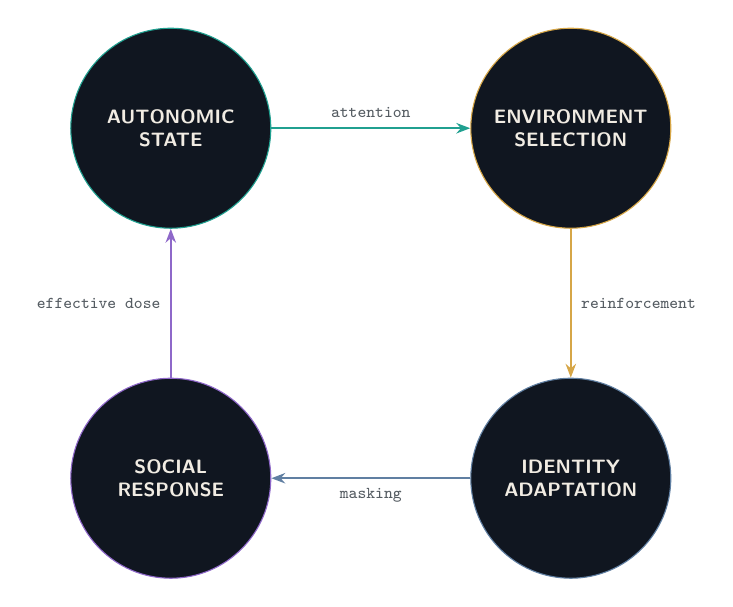
\begin{tikzpicture}[x=1in,y=1in]
\node[circle,draw=Teal,fill=Panel,text=Bone,minimum size=1.0in,align=center,font=\sffamily\bfseries\scriptsize] (a) at (0,0) {AUTONOMIC\\STATE};
\node[circle,draw=Gold,fill=Panel,text=Bone,minimum size=1.0in,align=center,font=\sffamily\bfseries\scriptsize] (e) at (2.0,0) {ENVIRONMENT\\SELECTION};
\node[circle,draw=Steel,fill=Panel,text=Bone,minimum size=1.0in,align=center,font=\sffamily\bfseries\scriptsize] (i) at (2.0,-1.75) {IDENTITY\\ADAPTATION};
\node[circle,draw=Violet,fill=Panel,text=Bone,minimum size=1.0in,align=center,font=\sffamily\bfseries\scriptsize] (s) at (0,-1.75) {SOCIAL\\RESPONSE};
\draw[-{Stealth[length=5pt]},Teal,line width=.85pt] (a)--node[above,font=\ttfamily\fontsize{5.8}{7}\selectfont,text=LightMuted]{attention}(e);
\draw[-{Stealth[length=5pt]},Gold,line width=.85pt] (e)--node[right,font=\ttfamily\fontsize{5.8}{7}\selectfont,text=LightMuted]{reinforcement}(i);
\draw[-{Stealth[length=5pt]},Steel,line width=.85pt] (i)--node[below,font=\ttfamily\fontsize{5.8}{7}\selectfont,text=LightMuted]{masking}(s);
\draw[-{Stealth[length=5pt]},Violet,line width=.85pt] (s)--node[left,font=\ttfamily\fontsize{5.8}{7}\selectfont,text=LightMuted]{effective dose}(a);
\end{tikzpicture}
\end{center}

\axiom{The phenotype is not the diagnosis. The diagnosis is one readout of the coupled system.}

\clearpage

% REGULATORY COUPLING HORIZON
\setfield{HORIZON HYPOTHESIS}{Gold}
\lightfieldbackground{Gold}{GoldPaper}
\kicker{THE HIGHER-ORDER AXIS}
\fieldtitle{Regulatory Coupling Orientation}

Regulatory Coupling Orientation describes where activation and regulation are preferentially recruited from. It is a spectrum, not a Hunter-versus-Farmer binary.

\begin{center}
\begin{tikzpicture}[x=1in,y=1in]
\draw[Ink!25,line width=1.1pt] (-2.5,0)--(2.5,0);
\draw[Oxide,line width=3pt] (-2.5,0)--(-.12,0);
\draw[Teal,line width=3pt] (.12,0)--(2.5,0);
\foreach \x in {-2.5,-1.25,0,1.25,2.5}{\draw[Ink!45] (\x,-.08)--(\x,.08);}
\node[align=center,font=\sffamily\bfseries\small,text=Oxide] at (-2.0,.45) {EXTERNAL-CUE\\DOMINANT};
\node[align=center,font=\sffamily\bfseries\small,text=Teal] at (2.0,.45) {INTERNALLY\\SUSTAINED};
\node[align=center,font=\fontsize{7.2}{8.7}\selectfont,text=Muted,text width=1.55in] at (-1.9,-.55) {novelty · motion · urgency\\immediate feedback · variance};
\node[align=center,font=\fontsize{7.2}{8.7}\selectfont,text=Muted,text width=1.55in] at (1.9,-.55) {routine · delayed reward\\low variance · self-generated activation};
\fill[Gold] (-.62,0) circle (4.2pt);
\draw[Gold,opacity=.38] (-.62,0) circle (.34in);
\end{tikzpicture}
\end{center}

\subhead{Regulatory Closure Bias: the measurable index}

\begin{evidencebox}{Gold}
\begin{equation*}
R_c=\log\!\left(\frac{G_{\mathrm{exo}}}{G_{\mathrm{endo}}}\right)
\end{equation*}
\small\color{Muted}
$G_{\mathrm{exo}}$ is regulatory gain produced through action on and feedback from the environment. $G_{\mathrm{endo}}$ is gain produced through internally maintained stabilization. Positive $R_c$ indicates exoregulatory bias; negative $R_c$ indicates endoregulatory bias.
\end{evidencebox}

\begin{fieldcard}{Teal}{ADHD-like dynamics \hfill \status{READOUT + RECURSIVE GAIN}{Teal}}
ADHD-like attention is modeled neither as sole root cause nor as decorative superpower. It can emerge from the full stack and feed back into it through environment selection, sleep timing, reward and urgency, stress exposure, autonomic state, and the consequences of prior action.
\end{fieldcard}

\subhead{What the orientation does not mean}

\begin{itemize}
  \item It is not locus of control, blame, motivation, or conscious preference.
  \item It does not claim that one phenotype is universally superior.
  \item It does not collapse RCCX, ADHD, trauma, chronotype, or D\k{a}browski into one cause.
  \item It predicts an interaction: phenotype $\times$ environment $\times$ available scaffolding.
\end{itemize}

\axiom{What appears to be internal instability may sometimes be a regulatory system deprived of the environmental surface through which it was built to close.}

\clearpage

% MOVEMENT III
\setfield{MOVEMENT III · REORGANIZATION}{Green}
\lightfieldbackground{Green}{GreenPaper}
\kicker{ONE SUBSTRATE · TWO TRAJECTORIES}
\fieldtitle{The Developmental Bifurcation}

\begin{center}
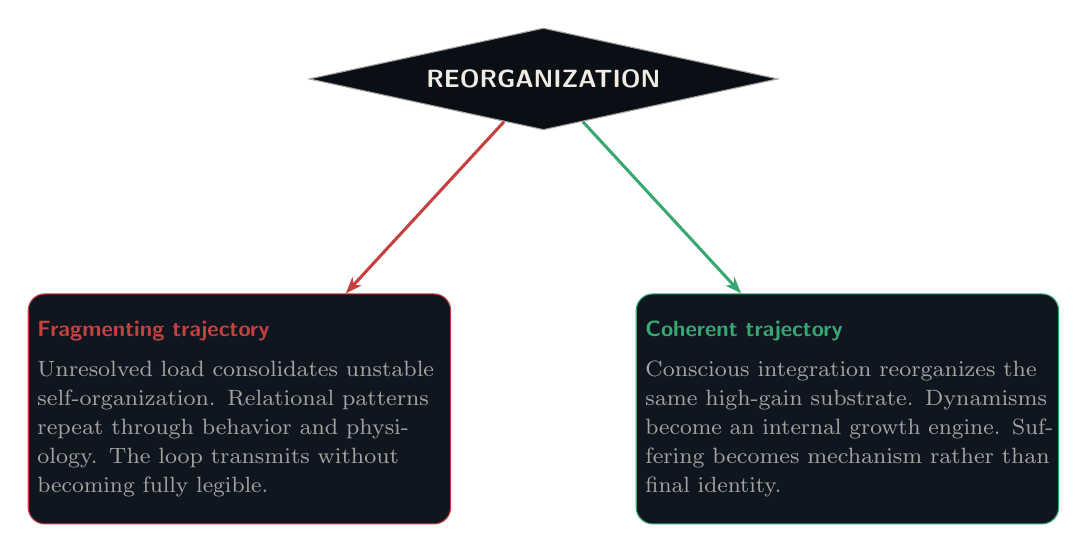
\begin{tikzpicture}[x=1in,y=1in,
  branch/.style={draw=#1,fill=Panel,rounded corners=6pt,text width=2.02in,minimum height=1.15in,align=left,font=\fontsize{8.3}{10.5}\selectfont,text=Muted},
  title/.style={font=\sffamily\bfseries\small}
]
\node[draw=Muted,fill=Deep,text=Bone,diamond,aspect=4.6,inner sep=5pt,align=center,font=\sffamily\bfseries\small] (b) at (0,0) {REORGANIZATION};
\node[branch=Red] (f) at (-1.52,-1.65) {\textcolor{Red}{\sffamily\bfseries Fragmenting trajectory}\\[4pt]Unresolved load consolidates unstable self-organization. Relational patterns repeat through behavior and physiology. The loop transmits without becoming fully legible.};
\node[branch=Green] (c) at (1.52,-1.65) {\textcolor{Green}{\sffamily\bfseries Coherent trajectory}\\[4pt]Conscious integration reorganizes the same high-gain substrate. Dynamisms become an internal growth engine. Suffering becomes mechanism rather than final identity.};
\draw[-{Stealth[length=6pt]},Red,line width=1.1pt] (b)--(f);
\draw[-{Stealth[length=6pt]},Green,line width=1.1pt] (b)--(c);
\end{tikzpicture}
\end{center}

\begin{fieldcard}{Gold}{Three-toggle convergence \hfill \status{ORIGINAL SYNTHESIS}{Gold}}
\textcolor{LightMuted}{\small All three must align for historically legible transformative output.}

\begin{description}[leftmargin=2.65em,labelwidth=2.25em,itemsep=.38em,style=multiline]
  \item[\textcolor{Gold}{T1}] \textbf{Orchestration magnitude} sets the ceiling: integrative, creative, perceptual, intellectual, emotional, and imaginative capacity.
  \item[\textcolor{Green}{T2}] \textbf{Reorganization direction} determines whether instability becomes fragmentation or greater coherence.
  \item[\textcolor{Teal}{T3a}] \textbf{Capacity conversion} requires health, discipline, closure, tools, access, collaborators, and capital.
  \item[\textcolor{Violet}{T3b}] \textbf{Dissemination} requires opportunity, uptake, networks, timing, and a channel into the historical record.
\end{description}
\end{fieldcard}

\begin{center}
\begin{tikzpicture}[node distance=.36in]
\node[draw=Gold!55,fill=Deep,text=Bone,rounded corners=4pt,text width=2.0in,minimum height=.56in,align=center,font=\sffamily\bfseries\scriptsize] (latent) {LATENT CEILING · UNREALIZED};
\node[draw=Gold!55,fill=Deep,text=Bone,rounded corners=4pt,text width=2.0in,minimum height=.56in,align=center,font=\sffamily\bfseries\scriptsize,below=of latent] (invis) {ACTUALIZED · HISTORICALLY INVISIBLE};
\coordinate (failuremid) at ($(latent)!0.5!(invis)$);
\node[draw=Gold,fill=Panel,text=Bone,rounded corners=5pt,text width=2.05in,minimum height=1.28in,align=center,font=\sffamily\bfseries\small] (conv) at ($(failuremid)+(3.0in,0)$) {MAGNITUDE\\$\times$ COHERENCE\\$\times$ CONVERSION\\$\times$ DISSEMINATION};
\draw[-{Stealth[length=5pt]},Gold!65,dashed] (latent)--(conv);
\draw[-{Stealth[length=5pt]},Gold!65,dashed] (invis)--(conv);
\node[below=.37in of conv,align=center,font=\sffamily\bfseries\small,text=Gold] (history) {HISTORICALLY LEGIBLE\\TRANSFORMATIVE OUTPUT};
\draw[-{Stealth[length=6pt]},Gold,line width=1pt] (conv)--(history);
\end{tikzpicture}
\end{center}

\axiom{Capacity is not impact until it survives conversion and enters the historical record.}

\clearpage

% COUPLED SCALES
\setfield{THE COUPLED MODELS}{Teal}
\lightfieldbackground{Teal}{BluePaper}
\kicker{ORGANISM / CIVILIZATION}
\fieldtitle{The Cascade and the Polymathic Singularity}

\begin{center}
\begin{tikzpicture}[x=1in,y=1in]
\node[draw=Violet,fill=Panel,text=Bone,rounded corners=7pt,text width=1.9in,minimum height=1.55in,align=center,font=\sffamily\bfseries\small] (inner) at (-1.55,0) {RCCX--HUNTER--D\k{A}BROWSKI\\CASCADE\\[6pt]\normalfont\fontsize{7.5}{9.5}\selectfont\color{Muted}within-person constitutional, developmental, physiological, and identity architecture};
\node[draw=Teal,fill=Panel,text=Bone,rounded corners=7pt,text width=1.9in,minimum height=1.55in,align=center,font=\sffamily\bfseries\small] (outer) at (1.55,0) {THE POLYMATHIC\\SINGULARITY\\[6pt]\normalfont\fontsize{7.5}{9.5}\selectfont\color{Muted}civilizational selection environment rotating around human-machine coupling};
\draw[-{Stealth[length=7pt]},Gold,line width=1.15pt] ([yshift=.20in]inner.east)--node[midway,above=-1pt,fill=BluePaper,inner sep=1.5pt,align=center,font=\ttfamily\fontsize{5.1}{6.1}\selectfont,text=Gold]{CONVERSION +\\DISSEMINATION} ([yshift=.20in]outer.west);
\draw[-{Stealth[length=7pt]},Oxide,line width=1.0pt] ([yshift=-.20in]outer.west)--node[midway,below=-1pt,fill=BluePaper,inner sep=1.5pt,align=center,font=\ttfamily\fontsize{5.1}{6.1}\selectfont,text=Oxide]{ALTERED\\PHENOTYPE PAYOFF} ([yshift=-.20in]inner.east);
\end{tikzpicture}
\end{center}

\subhead{The division of explanatory labor}

The cascade models the organism and its developmental history. The Polymathic Singularity models the environment changing which configurations gain leverage, visibility, and historical consequence. The two theories couple without proving one another.

\begin{fieldcard}{Gold}{AI enters at the conversion surface, not the root substrate \hfill \status{COUPLING CLAIM}{Gold}}
AI can hold structure, translate among representational languages, reduce implementation cost, and expand dissemination bandwidth. It can raise conversion capacity without creating the underlying orchestration magnitude:
\begin{equation*}
\kappa=\frac{\text{legible implemented output}}{\text{latent integrative capacity}}
\end{equation*}
It can also raise stimulation, branch proliferation, sleep displacement, and objective drift. The same coupling surface can amplify coherence or destabilize it.
\end{fieldcard}

\begin{fieldcard}{Teal}{The combined recursive loop \hfill \status{HORIZON SYNTHESIS}{Teal}}
\begin{center}\small
constitutional potential $\rightarrow$ developmental organization $\rightarrow$ cognitive phenotype\\
$\rightarrow$ human--AI coupling $\rightarrow$ environmental acceleration\\
$\rightarrow$ altered phenotype payoff $\rightarrow$ further niche construction
\end{center}
\end{fieldcard}

\subhead{The shared prediction}

High-exoregulatory, integrative profiles should improve disproportionately in responsive, AI-rich, project-based environments when the system supplies enough closure to prevent amplification from becoming branch proliferation. The causal variable is not diagnosis alone. It is the fit among architecture, environment, and conversion surface.

\axiom{The cascade explains how a ceiling becomes reachable. The singularity explains why the environment has begun paying for the climb.}

\clearpage

% EVIDENCE LEDGER
\setfield{EVIDENCE DISCIPLINE}{Violet}
\lightfieldbackground{Violet}{VioletPaper}
\kicker{THEORY WITHOUT COLLAPSED CERTAINTY}
\fieldtitle{Evidence and Source Ledger}

{\small\color{LightMuted}This model is intentionally integrative. The status grammar prevents established domains, supported mechanisms, developmental theory, integrative synthesis, and original horizon claims from collapsing into one undifferentiated certainty level. These are source anchors from the v3.1 handoff, not a finished bibliography.}\par

\begin{multicols}{2}
\raggedcolumns
\begin{evidencebox}{Gold}
\status{PROPOSED CLUSTER}{Gold}\par\textbf{Constitutional / RCCX}\par
\footnotesize\color{Muted}
Meglathery, RCCX theory materials.\par
Castori et al., hypermobility spectrum disorders and systemic involvement.\par
Tinkle et al. (2017), hEDS nosology and comorbidity landscape.
\end{evidencebox}

\begin{evidencebox}{Oxide}
\status{EVOLUTIONARY + ATTENTION}{Oxide}\par\textbf{Mismatch / state regulation}\par
\footnotesize\color{Muted}
Hartmann, \emph{Hunter in a Farmer's World}.\par
Sergeant (2005), cognitive-energetic model of ADHD.\par
Metin et al. (2012), event-rate meta-analysis.\par
Barack et al. (2024), ADHD traits and exploratory foraging.
\end{evidencebox}

\begin{evidencebox}{Green}
\status{SUPPORTED MECHANISM}{Green}\par\textbf{Epigenetic stress programming}\par
\footnotesize\color{Muted}
Meaney \& Szyf (2005), maternal care and glucocorticoid receptor methylation.\par
McGowan et al. (2009), childhood abuse and hippocampal NR3C1 methylation.\par
Klengel et al. (2013), FKBP5 $\times$ childhood trauma.\par
Yehuda et al. (2015), FKBP5 methylation across generations.
\end{evidencebox}

\begin{evidencebox}{Violet}
\status{DEVELOPMENTAL THEORY}{Violet}\par\textbf{D\k{a}browski / reorganization}\par
\footnotesize\color{Muted}
D\k{a}browski (1964), \emph{Positive Disintegration}.\par
D\k{a}browski (1972), \emph{Psychoneurosis Is Not an Illness}.\par
Mendaglio (2008, ed.), Theory of Positive Disintegration.
\end{evidencebox}

\begin{evidencebox}{Blue}
\status{ESTABLISHED + SYNTHESIS}{Blue}\par\textbf{Attachment / stress / autonomic}\par
\footnotesize\color{Muted}
Bowlby; Ainsworth; Main \& Hesse, attachment foundations.\par
McEwen, allostatic load.\par
Herman (1992), complex trauma.\par
Thayer \& Lane, neurovisceral integration.\par
Raj et al.; Eccles et al., POTS, hypermobility, and autonomic dysfunction.
\end{evidencebox}

\begin{evidencebox}{Steel}
\status{SUPPORTED PHENOMENON}{Steel}\par\textbf{Masking / social adaptation}\par
\footnotesize\color{Muted}
Jung, persona and shadow.\par
Cage et al. (2018), autistic camouflaging.\par
Hull et al. (2019), CAT-Q validation.\par
Lai et al., sex/gender differences in autism presentation.
\end{evidencebox}

\begin{evidencebox}{Teal}
\status{HORIZON DIRECTION}{Teal}\par\textbf{Chronotype / coupling}\par
\footnotesize\color{Muted}
Samson et al. (2017), chronotype diversity and nighttime coverage among Hadza.\par
Coogan \& McGowan (2017), ADHD circadian function and eveningness.\par
Yetish et al. (2015), sleep in three preindustrial societies.
\end{evidencebox}
\end{multicols}

\vfill
\begin{evidencebox}{Gold}
\textcolor{Gold}{\sffamily\bfseries NEXT FORMALIZATION TARGET}\quad
\small\color{Muted}Operationalize Regulatory Coupling Orientation independently of diagnosis; specify $G_{\mathrm{exo}}$ and $G_{\mathrm{endo}}$ across task environments; distinguish causal, modulatory, and recursive links; preregister phenotype $\times$ environment predictions; test when AI raises $\kappa$ and when it raises fragmentation instead.
\end{evidencebox}

\clearpage

% CODA
\color{Bone}
\thispagestyle{empty}
\begin{tikzpicture}[remember picture,overlay]
  \fill[Void] (current page.north west) rectangle (current page.south east);
  \coordinate (core) at ([xshift=1.40in,yshift=-.80in]current page.center);
  \draw[Gold,opacity=.72,line width=1.2pt] (core) circle (1.48in);
  \draw[Green,opacity=.45,line width=.7pt] (core) circle (1.03in);
  \draw[Violet,opacity=.32,line width=.45pt] (core) circle (.62in);
  \foreach \a/\c in {12/Gold,55/Green,98/Violet,144/Blue,192/Red,238/Oxide,284/Teal,332/Steel}{
    \draw[\c,opacity=.42,line width=.5pt] (core)--++(\a:2.05in);
    \fill[\c] ($(core)+(\a:2.05in)$) circle (2pt);
  }
  \draw[Red,line width=1.15pt] ([yshift=-2.9in]core)--++(-1.12in,-.66in);
  \draw[Green,line width=1.15pt] ([yshift=-2.9in]core)--++(1.12in,-.66in);
\end{tikzpicture}

\vspace*{.74in}
{\sffamily\bfseries\fontsize{7.4}{9}\selectfont\track{190}\textcolor{Gold}{THE CASCADE DOES NOT END AT THE DIAGNOSIS}}\par
\vspace{.42in}
{\sffamily\bfseries\fontsize{24}{28}\selectfont THE SAME SUBSTRATE\\CAN BECOME A CAGE,\\A COMPASS, OR A CEILING.}\par
\vspace{.28in}{\color{Oxide}\rule{1.05in}{3pt}}\par

\vspace{.30in}
\begin{minipage}{.76\linewidth}
{\fontsize{11.6}{16.2}\selectfont
Constitution changes the probability landscape. Development writes into regulation. Regulation reorganizes attention and action. Social response becomes additional environment. The system then reaches a real bifurcation: not between gifted and disordered, Hunter and Farmer, or sensitive and strong, but between trajectories that remain trapped inside their own recursive load and trajectories that learn to convert that load into coherence.

Even coherence is not enough. Capacity must survive conversion. Output must survive dissemination. The historical record does not contain every mind that reached the ceiling. It contains the minds whose ceilings acquired a surface through which they could become legible.}
\end{minipage}

\vfill
\begin{center}
{\sffamily\bfseries\fontsize{8.4}{11}\selectfont\track{48}
\textcolor{Red}{CONSTITUTION} \;\textcolor{Dim}{\(\rightarrow\)}\;
\textcolor{Oxide}{REGULATION} \;\textcolor{Dim}{\(\rightarrow\)}\;
\textcolor{Green}{REORGANIZATION}\\[.10in]
\textcolor{Dim}{\(\rightarrow\)}\;\textcolor{Gold}{HISTORICAL LEGIBILITY}}
\end{center}

\vspace{.44in}
{\sffamily\bfseries\fontsize{8}{9}\selectfont\track{115}\textcolor{Gold}{E.T. ELLIS}}
\hfill{\sffamily\fontsize{7}{8}\selectfont\textcolor{Dim}{RCCX--HUNTER--D\k{A}BROWSKI CASCADE · v3.2}}

\end{document}
